\chapter{Versionsverwaltung}\label{cha:Versionsverwaltung}
\section{Definition}\label{sec:Definition}
Versionsverwaltungssysteme sind auch bekannt als Versionskontrollsysteme (engl.
\acrlong{vcs}), Quellcode Verwaltung(engl. Source Control) oder
Revisionskontrollsysteme(engl. Revision Control System). Mit diesen Begriffen
sind Systeme, gemeint die es Entwicklern, Teams oder Organisationen erlauben
eine vollständige Historie mit allen Änderungen am Quellcode ihrer gemeinsam
entwickelten Software zu verwalten. Ausschlaggebend ist hierbei, dass für alle
Nutzer transparent wird, wer, wann und vor allem warum welche Änderungen
durchgeführt hat. Eine weitere wichtige Eigenschaft ist, dass es verschiedenen
Teams eine Zusammenarbeit an ggf. verschiedenen Teilen der Software
ermöglichti, ohne sich gegenseitig zu behindern\footnote{\label{dev:1}Das hängt
natürlich nicht nur von dem Versionskontrollsystem ab, sondern auch von dem
Sesign der entwickelten Software.  Diese wird i.d.R. eher modular aufgebaut, so
dass die Möglichkeit einer parallelen Entwicklung unterstützt
wird.}.\cite[S.~381]{cd}\\

In den nachvolgenden Abschnitten wird nicht im Detail auf alle existierende
Versionskontollsysteme eingegangen. Viel mehr wird ein kleiner Ausschnitt
weniger Systeme vorgestellt, der dazu dienen soll einen Überblick über die
grundlegende Entwicklung von Versionsverwaltungssystemen zu vermitteln.

\section{Geschichtliche Entwicklung}\label{sec:GeschichtlicheEntwicklung}
Das erste \gls{vcs:de} namens SCCS enstand 1972 und wurde von Marc J.  Rockkind
bei Bell Labs
geschrieben\footnote{\url{http://www.belllabs.com/}}\cite[S.~382]{cd}. Ab
diesem Zeitpunkt enstand eine Vielzahl von verschiedenen
Versionskontollsystemen. Als Alternative zu dem properitären \acrshort{sccs}
folgte Anfang 1980 das, von Walter F. Tichy an der Purdue University
entwickelte, erste \acrlong{OpenSource} Versionskontrollsystem
\acrfull{rcs}\cite{paper:rcs,link:rcs}. Ross Ridge veröffentlichte 1993 mit
einer Beta Version von \acrshort{mysc} einen freien Ersatz für \acrshort{sccs}.
In späteren Versionen wurde \acrshort{mysc} in \acrfull{cssc}
umbenannt\cite{link:cssc,link:mysc}. Alle drei Systeme finden in der Praxis nur
noch wenig Anwendungi. Daher wird diesbezüglich nicht auf weitere Details
eingegangen.

\subsection{CVS}\label{sec:cvs}
Das 1986 durch Dick Grune veröffentlichte \acrfull{cvs}, war das erste freie
Versionskontrollsystem mit einem zentralen \gls{repository}. Das wurde
erreicht, indem \acrshort{rcs}, mit Hilfe eines \gls{wrapper}, um eine
Client-/Serverkomponente erweitert wurde. Dadurch war es erstmals möglich, dass
mehrere Entwickler gleichzeitig an einem \gls{repository} und konkurrierend
anden selben Dateien arbeiten konnten. Neben den innovativen Ansätzen, gab es
hier aber noch einige technische Einschränkungen, die ein kollaboratives
Arbeiten erschwerten. Beispielsweise war die Nutzung des verbrauchten
Speicherplatzes nicht optimal. Das erzeugen von Abzweigungen (referenz fehlt!!
Branches) wurde durch einfaches Kopieren erreicht. Das war deshalb nicht nur
zeitaufwändig sondern verbrauchte auch entsprechend zusätzlichen Speicherplatz.
Ein späteres Zusammenführen (referenz fehlt!!! Mergen) dieser Zweige führte
daher zu Dateikonflikten und verursachte hierduch erheblichen Mehraufwand. Auch
gab es keine Funktonalität um Binärdateien zu verwalten so das der
Speicherplatz eher ineffizient genutzt wurde. Das Erstellen von
Tags\ref{sec:tag} wurde mit steigendem Inhalt des \glspl{repository} ebenfalls
immer zeitaufwändiger, da alle enthaltenen Dateien bearbeitet werden mussten.
Eine der, aus heutiger Sicht, größte Einschränkung war aber sicher die
Tatsache, dass Commits\ref{sec:commits} in das \gls{repository} nicht atomar
waren. Wurde die Übertragung der Dateien in das zentrale \gls{repository}
unterbrochen, so wurde dieses in einem inkonsistenten und nicht mehr nutzbaren
Zustand hinterlassen und musste administrativ repariert
werden.\cite[S.~382-383]{cd}

\subsection{SVN}\label{sec:svn}
Das Ziel des, als quasi Nachfolger zu \acrshort{cvs} entwickelten,
Versionsverwaltungssystems \acrfull{svn} war es, die technischen
Einschränkungen von \acrshort{cvs} zu beheben. Es wurde darauf geachtet, dass
es als Ersatz fungieren kann und das sich ein Umstieg sowohl aus
administriativer als auch aus Sicht eines Nutzers möglichst einfach gestaltet.
Das Benutzerinterface funktioniert daher ähnich zu \acrshort{cvs} so das
Entwickler sich nach einem Umstieg leichter zurecht finden. Als zentrale
Neuerung sind, im Gegensatz zu \acrshort{rcs} und \acrshort{sccs}, nicht mehr
die Dateien zentraler Bestandteil der Versionierung, sondern die sogenannte SVN
Revision. Jede Revision enthält einen eindeutigen Stand aller Dateien im
\gls{repository} zu einem bestimmten Zeitpunkt und ist global gültig und
eindeutig. Das ermöglicht direkte Vergleiche verschiedener Revisionen um
festzustellen welche Veränderungen zwischen zwei Revisionen durchgeführt
wurden. Alle Änderungen, wie z.B. das Kopieren, Hinzufügen oder Entfernen von
Dateien werden atomar durchgeführt. Im Gegensatz zu \acrshort{cvs} geht die
Historie, einer Datei nicht verloren wenn sie kopiert wird. Das Erstellen von
Tags oder Branches wurde ebenfalls verbessert. Hierzu wurde eine Konvention
eingeführt, die drei verschiedene Verzeichnisse innerhalb eines
\glspl{repository} vorgibt:
\begin{itemize}
\item \textbf{trunk}: Enthält die Revision, an der gemeinsam gearbeitet wird,
       und von der Branches und Tags erzeugt werden.
\item \textbf{tags}: Verzeichnis, in dem unterschiedliche Verzeichnisse als
       Tags erzeugt werden, die von einer bestimmten Revision erzeugt werden.
\item \textbf{branches}: Ein Verzeichnis, in dem unterschiedliche Ordner als
      Abzweigungen angelegt werden. Auf diesen Abzweigungen kann unabhängig von
      \textit{trunk} gearbeitet werden.
\end{itemize}
Die o.a. Verzeichnisse bzw. Tags\ref{sec:tag} und \ref{sec:branches}Branches
sind lediglich Zeiger auf eine bestimmte Revision und die Trennung dazwischen
ist nur eine Konvention. So werden Tags und Branches erzeugt in dem ein
Verzeichnis angelegt wird und der Inhalt von \textit{trunk} kopiert wird. Das
führt auch zu einem der Probleme bei dem Arbeiten mit \acrlong{svn}. Tags sind
nicht eindeutig und veränderbar.  So macht SVN technisch keinen Unterschied
zwischen \textit{trunk}, \textit{tags}, \textit{branches} oder einem beliebigen
anderen Verzeichnis. Alle können in der gleichen Art und Weise bearbeitet
werden. Ein großer Vorteil von \acrshort{svn} zu vorherigen
Versionskontrollsystemen ist, das mit \acrshort{svn} auch gearbeitet werden
kann, wenn das Netzwerk nicht zur Verfügung steht. Alle Änderungen an Dateien
werden i.d.R. erstmal auf einer lokalen Kopie durchgeführt und mit einem
separaten Kommando an das zentrale Repository gesendet. Als weitere
Funktionalität seien noch sogenannte Externals erwähnt, die es erstmals
ermöglichen Inhalte von anderen Repositorys einzubinden. Dies kann nützlich
sein, um Abhängigkeiten zwischen unterschiedlicher Software oder
\glspl{repository} abzubilden und Binärdateien auszulagern. \acrshort{svn}
stellte zwar eine erhebliche Neuerung gegenüber \acrshort{cvs} dar, hatte aber
aufgrund der zusätzlichen Client-/Server Komponente einige neue Probleme. So
waren z.B. zwar die Aktionen aufseiten des zentralen \glspl{repository} atomar,
aber nicht aufseiten des Clients. So das hier, bei unvorhergesehenen Fehlern,
wieder Inkonsistenzen entstehen konnten. Des Weiteren verwaltet \acrshort{svn}
mit Hilfe eines Unterordners \textit{.svn} in jedem enthaltenen Verzeichnis die
Verwaltungsinformationen des selbigen. Das ermöglicht eine unabhängige
Verwaltung aller Verzeichnisse untereinander und führt ggf. dazu, dass die
lokale Kopie eine Summe aus unterschiedlicher Revisionen verschiedener
Unterordnern ist und keinen eindeutigen Versionsstand repräsentiert.  Die o.a.
Abschnitt stellt aber nur einen Auszug der Vor- und Nachteile von SVN dar. Auf
eine weitere Ausführung wird aus Platzgründen verzichtet und kann in
einschlägiger Literatur nachgelesen werden.\cite[S.~383-385]{cd}

\subsection{Git}\label{git}
Git ist ein verteiltes bzw. dezentrales \acrlong{vcs:de}. Es wurde von Linux
Torvalds und Junio Hamano entwickelt und ist für gängige Plattformen wie
Linux, BSD, Windows u.a. verfügbar. Der Name Git kommt nach einem Zitat von
Linus Torvalds wie folgt zustande\cite{link:gitfaq}:

\begin{center}
\textit{\glqq{}I'm an egotistical bastard, and I name all my projects after
myself. First 'Linux', now 'Git'\grqq{}}\\
\end{center}

Alternativ stellt Linus Torvalds, etwas schertzhaft, noch weitere Varianten als Übersetzung des
Akronyms \textit{Git} zur Verf\-ügung\cite{link:gitfaq}:

\begin{itemize}
  \item \textit{\glqq{}Random three-letter combination that is pronounceable, and not
  actually used by any common UNIX command. The fact that it is a
  mispronunciation of "get" may or may not be relevant.\grqq{}}
  \item \textit{\glqq{}Stupid. Contemptible and despicable. Simple. Take your pick from the
  dictionary of slang.\grqq{}}
  \item \textit{\glqq{}Global information tracker": you're in a good mood, and it actually
  works for you. Angels sing and light suddenly fills the room.\grqq{}}
  \item \textit{\glqq{}Goddamn idiotic truckload of sh*t": when it breaks\grqq{}}
\end{itemize}

Linus Torvalds nutzte ursprünglich als Versionsverwaltung das kommerzielle System BitKeeper für
die Entwicklung am Linux
Kernel\footnote{\url{https://git.kernel.org/pub/scm/linux/kernel/git/torvalds/linux.git}}.
Nach Unstimmigkeiten mit dem Hersteller von BitKeeper entschloss Linux Tovalds
sich dazu, ein neues \gls{vcs:de} zu schreiben. Dieses sollte weit mehr als
eine Alternative zu den bisherigen sein\cite[S.~13]{gitosp}. So lautete 2005
eine Aussage von Linus Torvalds zu \acrshort{cvs}\cite[S.~385]{cd}:

\begin{center}
\textit{\glqq{}There is no way to do CVS right\grqq{}}\\
\end{center}

Neben dem Beheben der Probleme mit denen die populären Systeme (Abschnitt
\ref{sec:svn} und \ref{sec:cvs}) zu kämpfen hatten sollte das zentrale
Augenmerk auf Geschwindigkeit und Integrität liegen. Schon Wenige Wochen nach
dem Start mit der Arbeit an Git konnten die ersten Versionen bereits Quellkode
verwalten. Die grundlegenden Konzepte sind bis heute gleich geblieben. Die
spätere erfolgreiche Migration und Verwaltung des Linux Kernel
\glspl{repository} mit Git, führte zu einem hohen Ansehen und einer starken
Verbreitung von Git. Die Anforderungen an ein \acrlong{vcs:de}, um den Linux Kernel
mit über 1000 Entwicklern zu verwalten sind immens. Allein zwischen zwei
Versionen finden sich mehrere hunderttausend Änderungen in über 1000 Dateien
und etliche Merges zwischen verschiedenen Branches (Abschnitt
\ref{cha:kernel}). Git selbst ist heutzutage, insbesondere in großen Projekten
kaum mehr wegzudenken.\cite[S.~13]{gitosp}

\section{Kollaboration}\label{sec:collaboration}
Die Möglichkeit, Änderungen transparent und nachvollziehbar in einem
\gls{repository} zu speichern und bei Bedarf wieder zurückzunehmen, Stände die
zu unterschiedlichen Zeitpunkten erzeugt wurden zu vergleichen,
zusammenzuführen und Teile davon wieder herzustellen, ermöglicht es die
Zusammenarbeit in Teams oder Organisationen erheblich zu verbessern. Alle
Beteiligten werden damit konfrontiert, dass mehrere Personen und Teams an
gleichen Inhalten zur gleichen Zeit arbeiten müssen. Das verbessert den Umgang
mit Konflikten, seien sie technischer oder organisatorischer Art, die eben
durch eine solche Zusammenarbeit enstehen können. Der frühe Einsatz eines
Versionsverwaltungssystems sollte als eine gute Angewohnheit angesehen werden,
die einen positiven Einfluss auf die Zusammenarbeit hat. Da nicht alle Systeme
die gleichen Funktionen unterstützen, sollte bei der Auswahl des einzusetzenden
Systems darauf geachtet werden, welche Eigenschaften der Zusammenarbeit
gefördert werden sollen. So könnten das nach Jennifer Davis und Katherine
Daniels in \cite[S.~178]{effdo} z.B. folgende sein:

\begin{itemize}
\item Erstellen und Abzweigen von Repositories,
\item Beitragen zu Repositories bwz. das Verwalten von Beiträgen,
\item Festlegen von Prozessen oder
\item das Verwalten von Berechtigungen innerhalb von Repositories.
\end{itemize}

Der Einsatz eines \glspl{vcs:de} hat auch einen positiven Einfluss auf Risiken,
die beispielsweise bei Änderungen an einer produktiven Softwareplattform (z.B.
eines Internetportals) enstehen. Hierdurch wird es möglich, im Fehlerfall eine
frühere Version der Software wieder einzusetzen und solche Risiken zu
verringern.\cite[S.~178]{effdo}

Ein \acrlong{vcs:de} ist auch nicht ausschließlich zum Versionieren von Quellcode
geeignet. Eine Aussage von Jez Humble und David Farley in \cite[S.~33]{cd}
lautet hierzu:

\begin{center}
\glqq{}Keep Absolutely Everything in Version Control\grqq{}
\end{center}

Jede Datei, die benötigt wird um die Software reproduzierbar zu erzeugen und zu
verwalten sollte sich unter Versionskontolle befinden. Das können beliebige
Dateien sein, wie z.B.

\begin{itemize}
\item Quellcode,
\item Tests,
\item Skripte zum Kompilieren oder zur Datenbankverwaltung,
\item Bibliotheken oder
\item Konfigurationen.
\end{itemize}

So können neue Mitarbeiter schnell in Teams integriert werden und ein
effizienter Start wird gefördert. Es ist ebenso wichtig, dass alle benötigten
Informationen unter Versionskontolle stehen und allen Beteiligten zur Verfügung
stehen. Hierzu gehören neben Dokumentationen beispielsweise Projekt- und
Releasepläne der Manager oder Dokumente über durchgeführte Analysen. Darüber
hinaus sollten auch externe Abhängigkeiten mit verwaltet werden. So könnten
hier ebenso

\begin{itemize}
\item DNS Zonendateien,
\item Regeln für eine Firewall oder
\item die Konfiguration für eine Entwicklungsumgebung mit versioniert werden.
\end{itemize}

Im Kern alles was nötig, ist um Umgebungen (insbesondere produktive\footnote{Es
gibt sicher eine Vielzahl von Szenarien die es als wirtschaftlich arbeitendes
Unternehmen erfordern, zu so etwas in der Lage zu sein. Ausgenommen vielleicht
Anbieter einschlägiger Suchmaschinen die beispielsweise nicht vom Abbrennen
eines einzelnen Datenzentrums abhängig sind.}) von Grund auf neu zu erzeugen.
Erst wenn all diese Informationen und Dateien, die sich über die Zeit
verändern, in einem Versionskontrollsystem verwaltet werden ist es möglich das
Projekt oder die Software von/zu einem beliebigen Zeitpunkt in der Historie
wieder herzustellen.\cite[S.~33]{cd}

\section{Allgemeine Grundlagen}\label{sec:Grundlagen}
Aus den vorhergehenden Abschnitten lässt sich zusammenfassend feststellen, dass
es aus Sicht der Benutzer, für den gemeinsamen Zugriff auf Dateien, bestimmte
Anforderungen gibt. Nach \cite[S.~37]{hagen:1678} bestehen Forderungen nach
\textbf{Aktualität}, \textbf{Konsistenz}, \textbf{Isolation},
\textbf{Integration}, \textbf{Gruppenwahrnehmung} und
\textbf{Nachvollziehbarkeit}. So sollen Entwickler in der Lage sein immer an
einer gültigen Fassung einer Datei zu arbeiten als sei diese Datei exklusiv für
sie reserviert sowie die eigenen Änderungen daran so wieder zu integrieren das
eine Nachvollziehbarkeit mit einer Änderungshistorie, die wenigstens Namen und
Datum enthält, gewährleistet ist. Wie sich, mit Git, eine Umsetzung dieser
Forderungen in der Praxis darstellt wird in den folgenden Unterkapiteln
gezeigt. Vorher aber, werden noch einige benötigte Grundbegriffe erläutert.

\subsection{Commit}\label{sec:commit}
Werden Veränderungen am Repository durchgeführt bzw. an den darin enthaltenen
Dateien werden diese als Commits gespeichert. Hierzu werden die einzelnen
Veränderungen and Dateien oder Metadaten z.B. löschen, hinzufügen oder
Veränderungen and Dateiberechtigungen durch den Autor, mit verschiedenen
Kommandos, zusammengefasst und mit Namen, Zeitpunkt und Beschreibung als Commit
dem Repository hinzugefügt. Unter Git referenziert ein Commit immer einen
eindeutigen Zustand aller verwalteten Dateien. Diese Referenz enhält eine
inhaltsabhänigige eindeutige 160-Bit lange Prüfsumme, die auch als
\textit{Commit-ID} bezeichnet wird(siehe Abschnitt \ref{sec:kernel},
\pageref{sec:kernel}). Die inhaltsabhängige Prüfsumme gewährleistet auch das
Inhalte nachträglich nicht unbemerkt verändert werden können. Die Prüfsumme
wird mit dem \textit{Secure Hash Algotithm} (\gls{SHA-1})
erzeugt.\cite[S.~20-21]{gitos}

\subsection{Tag}\label{sec:tag}
Die meisten Versionskontollsysteme\ref{cha:Versionskontrollsysteme} benutzten
Tags um bestimmte Stände des Repositorys mit Namen zu versehen. Die übliche
Anwendung sind Versionsnummern wie z.B. 2.6.12-rc2( Abschnitt
\ref{sec:kernel}), v1.0 oder ähnliche. Unter Git sind Tags
lediglich symbolische Namen für Referenzen zu einzelnen Commits. Es gibt hier
zwei verschiedene Arten von Commits. Zum einen leichtgewichtige Tags
(\textit{lightweight tags}) die keine weiteren Informationen ausser der
Versionsnummer enthalten und ausführlichere Tags (\textit{annotated}) die
darüber hinaus noch Metadaten wie Autor, Beschreibung oder ggf. eine Signatur
mit GPG enthalten.\cite[S.~48]{progit}

\subsection{Branch}\label{sec:branches}
Ein Repository enthält i.d.R. mindestens einen zentralen Zweig(Branch) auf dem
die Entwicklungsarbeit stattfindet. Ein Abzweig an einer bestimmten Stelle zu
einem bestimmten Zeitpunkt erzeigt einen neuen Branch. Dieser Abzweig kann von
dem zentralen oder einem andern Branch erfolgen. Wie diese Branches erzeugt
werden ist abbhängig von dem eingesetzten Versionskonrollsystem. So wird unter
\acrshort{svn} oder \acrshort{cvs} der Branch mittels eines Kopiervorgangs
erzeugt(Abschnitt \ref{sec:cvs}\ref{sec:svn} und unter Git über eine lediglich
über eine symbolische Referenz. Häufig werden Branches verwendet um Features zu
entwickeln, Releases zu erzeugen oder Bugfixes an bestehenden Versionen
durchzuführen\cite[S.~21]. Um effizient mit Branches umzugehen gibt es
verschiedene Strategien so wird von Jez Humble und David Farley in
\cite[S.~408-412]{cd} auf Releasebranches, Featurebranches, Teambranches oder
einer Entwicklung mit nur einem Hauptbranch\footnote{Umgangsprachlich werden
verschiedene Begriffe für diesen Branch benutzt. So sind Begriffe wie z.b.
Trunk, Masterbranch oder Mainlinebranch nicht unüblich. Gemeint ist hiermit
i.d.R. aber immer der zentrale Branch der Standardmäßig von dem genutzen
\acrlong{vcs} vorgesehen ist. Für \acrshort{svn} ist das z.B. per Konvention
das Verzeichnis \textit{trunk} und unter Git einfach die Referenz auf den Namen
\textit{master}.} eingegangen.

\subsection{Merge}\label{sec:merge}
Wenn wie in dem Abschnitt \ref{sec:collaboration} auf Seite
\pageref{sec:collaboration} mehrere Entwickler in dem \gls{repository} arbeiten
entstehen an einer gemeinsamen Basis häufig paralelle Abzweige. An diesen wird
gleichzeitig gearbeitet und dadurch laufen diese Zweige u.U. auseinander. Das
spätere wieder Zusammenführen dieser Zweige bezeichnet man als Merge. Git
bietet hier mit \textit{merge}, \textit{mergetool}, \textit{rebase} und
\textit{cherry-pick} eine umfangreiche Unterstüzung\cite[S.~vii]{gitwf}. Beim
zusammenführen der beiden Zweige, z.B. \textit{topic} und \textit{master}
ensteht wie in Abbildung \ref{fig:merge} gezeigt ein sogenannter Merge-Commit.
Dieser hat seinen Ursprung in den beiden vorhergehenden Knoten dieser Zweige.

\begin{figure}[hb]
  \centering
  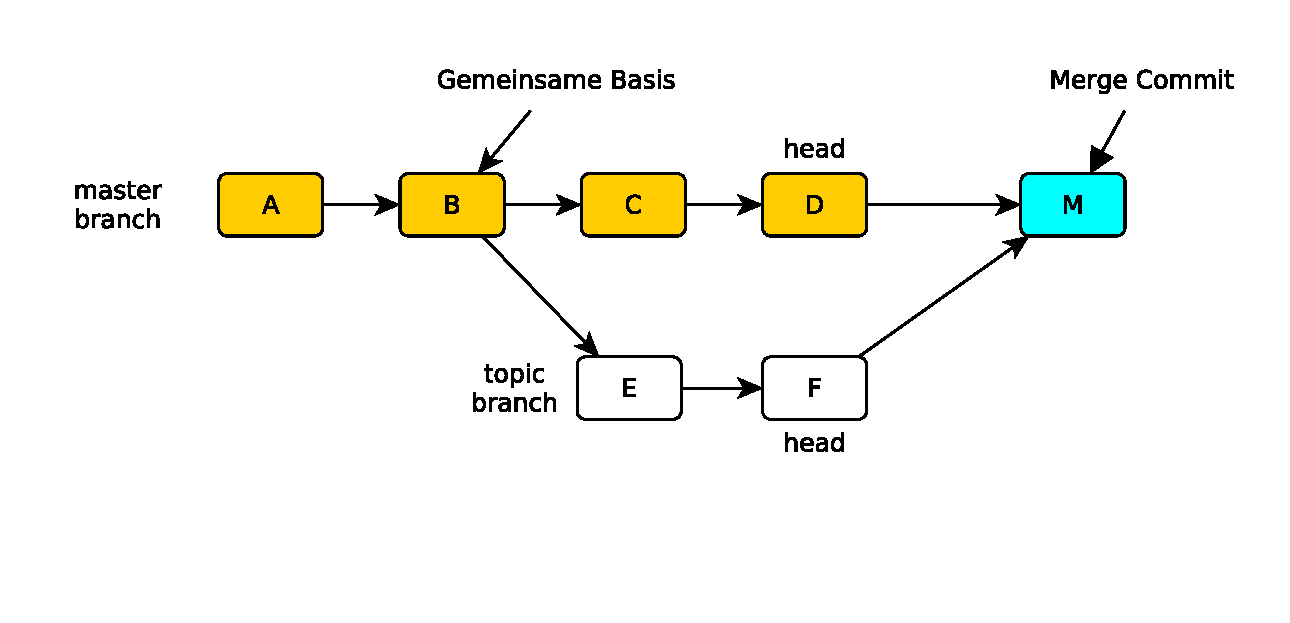
\includegraphics[scale=0.60]{images/merge.eps}
  \caption{Zusammenführen zwei Branches}
  \label{fig:merge}
\end{figure}

Komplexere Szenarien erlauben es mit git auch Merges aus mehr als zwei Branches
zu erzeugen z.b. sogenannte \textit{tree-way-merges} oder
\textit{octopus-merges}\cite[S.~87]{gitosp}. Git ermöglicht es auch Zeige aus verschiedenen
Repositorys zusammenzuführen. So gibt es nach \cite[3]{gitwf} noch die
Möglichkeit Repositorys nach spezielleren Funktionen zu unterteilen. So kann
ein dediziertes \textit{Blessed Repositorys} ausschliesslich für das erstellen
von Versionen der erzeugten Software genutzt werden. Die Änderungen können aus
einem \textit{Fork Repository} importiert werden. Das \textit{Fork Repository}
dient zur Entkopplung des Haupt-Repositorys. So können größere Umbauten, Merges
oder Features unabhängig vom Haupt-Repository entwickelt
werden\cite[S.~123]{gitwf}. Eine vergleichbare Vorgehensweise findet man im
Repository des Linux Kernels\cite{link:linuxgit} aus Abschnitt \ref{sec:kernel}
auf Seite \pageref{sec:kernel}.

\subsection{Repository}\label{sec:repository}
Das Repository ist ein Datenspeicher in dem gemeinsame Dateien eines Projekts
durch das \acrlong{vcs:de} verwaltet werden. Der Benutzer kann hier Dateien
z.B. Hinzufügen, Entfernen oder Manipulieren. Das  \acrlong{vcs:de} erzeugt,
für alle in Commits\ref{label:commit} zusammengefasten Anderungen, eine
Historie mit den durchgeführten Änderungen\cite[S.~38]{hagen:1678}.

\subsection{HEAD}\label{sec:head}
Eine Referenz auf den letzten Commit im aktuellen Repository bzw. Branch
verweist. Hier muss zwischen verschiedenen Versionskontrollsystemen
unterschieden werden. So ist unter Git die HEAD Version eine symbolische
Referenz auf die letzte Version des aktuell lokal genutzten Branches. Diese ist
also abhängig von den gerade vorhandenen Daten im Working Tree von
Git\cite[S.~20]{gitosp}. Für SVN hingegen bezeichnet HEAD die letzte
veröffentlichte Version im Repository.

\section{Arten von Versionsverwaltungssystemen}
\subsection{Lokal}\label{sec:local}
Frühe Versionskontrollsysteme wie \acrshort{rcs} oder \acrshort{rcs} arbeiten
ausschliesslich auf dem lokalen Dateisystem und sind nicht dafür entwickelt ein
kollaboratives Arbeiten zu unterstützen. Hier geht es auschliesslich darum
einem Entwickler eine lokale Versionsverwaltung zur ermöglichen. Die Inhalte
können weiteren Personen nicht mit Mitteln des \acrlong{vcs:de} zur Verfügung
gestellt werden.

\subsection{Zentral}\label{sec:central}
Versionskontrollsysteme wie \acrshort{svn} oder \acrshort{cvs} stellen ein
zenrales \gls{repository} mit hilfe einer Serverkomponente zur Verfügung.
Entsprechend dazu gibt es für verschiedene Betriebsysteme Clientkomponenten. So
gibt es für Linux oder andere Unix-derivate i.d.R. frei verfügbare Server- und
Clientkomponenten die zum Teil grafisch als auch auf einem Terminal zu bedienen
sind. Die Kommunikation der Clientkomponente mit dem Server erfolgt i.d.R.
direkt. Das bedeutet der Benutzer holt mit dem Client die Dokumente aus dem
zentralen Repository, führt seine Änderungen durch und fasst diese in einem
Commit\ref{commit} zusammen. Hierfür stellt das \acrlong{vcs:de} entsprechende
Unterstützung bereit. So z.b. für die o.a. Versionskontrollsysteme einen Befehl
\textit{checkout} zum holen der Dokumente und  \textit{commit} zum zusammenfassen
und gleichzeitigem übertragen an die Serverkomponente. Die Bearbeitung der
Dokumente im lokalen \ref{sec:repository} erfolgt i.d.R. mit unabhängigen
Werkzeugen.\cite[S.~38-40]{hagen:1678}

\subsection{Verteilt}\label{sec:decentral}
Versionskonrollsysteme die Verteilt arbeiten werden im englischen
\acrfull{dvcs} genannt und zeichnen sich dadurch aus das der Benutzer, lokal,
ein vollwertiges \gls{repository} zur Verfügung hat ohne das eine
Serverkomponente ein zentrales zur Verfügung stellen muss. Das ist aber nicht
zu verwechseln mit lokalen Versionskontrollsystemen\ref{sec:local} wie
\acrshort{rcs} oder \acrshort{sccs}. Der Unterschied ist das verteilte Systeme
das gleichzeitige Arbeiten von mehreren Usern stärker unterstützen als zentrale
\acrshort{vcs:de}. Dabei ist es unerheblich ob Benutzer gleichzeitig, an
mehreren Branches, an verschiedenen Repositorys und/oder an den geleichen
Dateien arbeiten oder nicht.\cite[S.~393-394]{cd}

Ein Auszug aus den von Jez Humble und David Farley in \cite[S.~393-394]{cd}
beschriebenen Eigenschaften eines \acrshort{dvcs} lautet wie folgt:

\begin{itemize}
\item Es ist keine Serverkomponente nötig um einen Commit in ein lokales
\gls{repository} durchzuführen.
\item \glspl{repository} verschiedener Benutzer und Quellen können miteinander
verbunden werden und deren Inhalte verglichen, integriert oder verändert werden. 
\item Um Veränderungen durchzuführen und in einem \ref{commit} zusammenzufassen
ist unerheblich ob eine Netzwerkverbindung zu einer möglichen Quelle besteht
\item Änderungen können an eingeschränkte Nutzergruppen veröffentlicht werden
ohne das jemand gezwungen ist diese zu übernehmen.
\item Dadurch das jeder Benutzer eine eigene vollwertige Kopie des
\glspl{repository} hat, sind \acrshort{dvcs} robuster gegenüber Datenverluste.
Darüberhinaus können Benutzer dadurch lokal branches anlegen und ggf.
Experimente machen ohne diese immer in ein zentrales Repository zu übertragen.
Das sorgt zusätzlich für eine bessere Skalierbarbeit.
\item Commits, Branches und Tags können lokal sortiert geordnet und ggf.
Zusammengefasst werden bevor die Übertragung in ein gemeinsam genutztes
\gls{repository} durchgeführt wird.\footnote{Das wird im Kontext von Git als
\textit{rebase} bezeichnet.}
\end{itemize}

Im Gegensatz zu zentralen (Abschnitt \ref{sec:central}) Versionskontrollsystemen erfolgt das
erzeugen eines \glspl{commit}\ref{sec:commit} lokal und die Übertragung in ein ggf.
weiteres \gls{repository} mit einem zusäztlichem Befehl \textit{push}. Dabei
können die Daten beliebig oft in weitere \glspl{repository} übertragen werden.

\subsection{Streaming}\label{sec:streaming}
An dieser Stelle sei noch grob auf Versionskontrollsysteme eingegangen die auf
Datenströmen basieren. Ein populäres Beispiel ist das kommerziell vermarktete
ClearCase entwickelt von IBM. Das zentrale Merkmal ist hier das
Branches\ref{sec:branch} durch sogenannte Streams ersetzt wurden.
Das ermöglicht eine Baumstruktur von abhängigen Abzweigen die durch eine
Vererbungsstruktur verbunden sind. Es können Änderungen innerhalb eines
Arbeitsbereichs durchgeführt werden ohne andere Benutzer zu bereinflussen. Nach
Abschluss dieser Arbeiten können diese veröffentlicht bzw. \textit{promoted}
werden. Diese werden dann allen abhängigen Streams gleichzeitig zur Verfügung
gestellt. Das kann hilfreich sein um z.B. grundlegende Softwarebibliotheken
auszutauschen oder wichtige Fehlerbehebungen durchzuführen. In herkömmlichen
\acrshort{vcs:de} müssen solche Änderungen einzeln auf jeden Branch übertragen
werden.
